% Draft. Compile with:
%   pdflatex main && bibtex main && pdflatex main && pdflatex main
% Figures are read from ../figures/, produced by ../experiments/make_figures.py.
\documentclass[11pt]{article}

\usepackage[margin=1in]{geometry}
\usepackage{amsmath,amssymb,amsthm}
\usepackage{graphicx}
\usepackage{booktabs}
\usepackage[round,authoryear]{natbib}
\usepackage[hidelinks]{hyperref}

\graphicspath{{../figures/}}

\newcommand{\E}{\mathbb{E}}
\newcommand{\KL}{\mathrm{KL}}
\newcommand{\F}{\mathcal{F}}
\newcommand{\G}{\mathcal{G}}

\newtheorem{theorem}{Theorem}
\newtheorem{proposition}{Proposition}
\newtheorem{corollary}{Corollary}
\theoremstyle{remark}
\newtheorem{remark}{Remark}

\title{Betting against the simulator: anytime-valid criticism of\\
generative models and digital twins under adaptive control}

\author{Elena Bortolato\\ CUNEF Universidad}

\date{Draft --- \today}

\begin{document}
\maketitle

\begin{abstract}
Simulators, generative models and digital twins are increasingly used inside
decision loops, where actions are chosen from the data and the analyst can
only \emph{sample} from the model. We ask how to monitor, as data arrive,
whether reality has departed from such a model, with a false-alarm guarantee
that holds at every time and under any stopping rule. At each step we draw $M$
fresh samples from the simulator for the context and action actually taken,
score them together with the real observation using a score learned from the
past, and bet on the rank-like statistic
$(M+1)\,T(X_t)/\{T(X_t) + \sum_j T(Y_{t,j})\}$. By exchangeability, the bet has
conditional null expectation exactly one, whatever the learner, so the running
wealth is a test martingale. No density is evaluated. We show that simulating
conditionally on the action is sufficient for validity under arbitrary
adaptive policies and that it cannot be dropped. We then characterise power. The
growth rate is bounded by $\KL(Q\|P)$, equals $\KL(Q\|P) - \KL(Q\|\hat Q)$ with
an unlimited simulation budget, where $\hat Q$ is the null tilted by the score,
and loses a factor $M/(M+1)$ for local alternatives. With posterior predictive
scores the infinite-budget process is a Bayes factor, and we compute the
posterior online with one natural-gradient step of the Bayesian learning rule
per observation. In experiments with a drifting generative model and a
Thompson-sampling bandit checked against a digital twin, the method keeps
false alarms below the nominal level, whereas using a learned ratio directly
as the bet gives up to 59\% false alarms, and re-running fixed-sample tests
32--39\%, at $\alpha = 0.05$.
\end{abstract}

%======================================================================
\section{Introduction}\label{sec:intro}
%======================================================================

A simulator is often trusted only as long as it agrees with the system it
represents. Digital twins of manufacturing lines and hospitals are
re-initialised from the observed state and used to choose the next
intervention; agent-based and epidemic simulators drive policy while new
cases are recorded; generative models are deployed and their outputs compared
with fresh real data; and adaptive experiments allocate treatments using the
responses seen so far. In each case the same question recurs as data arrive:
\emph{is the system still behaving as the model says it should?} Three
features make it hard. The model is usually available only as a sampler, with
no tractable likelihood. The data arrive one at a time, and the analyst wants
to look after every observation and stop at the first convincing evidence.
And the observations are not exchangeable, because actions are chosen from
the data.

Standard tools each fail one of these requirements. Fixed-sample
goodness-of-fit tests lose their error guarantee when they are recomputed
after every observation. Likelihood-ratio e-processes are anytime-valid but
need the null density. A classifier trained to separate real from simulated
data estimates the density ratio \citep{thomas2022lfire}, but its estimate is
not calibrated, and betting with it directly is not valid. Conformal test
martingales \citep{vovk2003testing,vovk2021testing} monitor a stream without
a model, but they test whether the stream is exchangeable, not whether it
agrees with a simulator.

We propose a simple construction. At each step, draw $M$ samples from the
simulator \emph{for the same context and action as the real observation},
score all $M+1$ points with a score fitted on the past, and bet the share of
the real point in the total score, rescaled by $M+1$. Under the null the real
point is exchangeable with the simulated ones, so the bet is fair for every
score; the product of bets is a test martingale; and Ville's inequality gives
an anytime-valid test. The learner affects power but never validity.

\paragraph{Contributions.}
\begin{enumerate}
  \item \textbf{Validity under adaptive control} (Theorem~\ref{thm:valid}).
        The Monte Carlo e-process is a test martingale under any adaptive
        policy, provided the simulator is run conditionally on the action
        taken. Proposition~\ref{prop:necessary} shows that this condition
        cannot be dropped: simulating from the wrong action mixture makes
        the wealth grow under the null.
  \item \textbf{Power} (Theorem~\ref{thm:growth}). The growth rate is at most
        $\KL(Q\|P)$; with an unlimited budget it equals
        $\KL(Q\|P) - \KL(Q\|\hat Q)$, where $\hat Q$ is the null tilted by the
        score; a non-asymptotic bound controls finite budgets; and for local
        alternatives the finite-budget efficiency is exactly $M/(M+1)$ to
        second order. A finite budget also tempers overconfident scores.
  \item \textbf{Bayesian predictive scores} (Proposition~\ref{prop:bayes}).
        With posterior predictive scores under an exponential tilt of the
        simulator, the infinite-budget process is the Bayes factor of the
        tilted family against the simulator, so the total learning cost is
        $(d/2)\log t$. We compute the posterior online with the Bayesian
        learning rule \citep{khan2023bayesian,jones2024bong}. Its
        approximations cannot affect validity.
  \item \textbf{Experiments} on a drifting generative model, a
        Thompson-sampling bandit checked against a digital twin, and a
        numerical check of the theory.
\end{enumerate}

The single-step argument is the exchangeability argument of Monte Carlo tests
\citep{besag1989generalized}, and betting on a stream is the framework of
\citet{shafer2021testing} and \citet{ramdas2023game}. Per-step sampling from a
known conditional null already appears in model-X sequential testing of
conditional independence \citep{shaer2023modelx}, and Besag--Clifford
e-values have recently been developed for unnormalised models
\citep{dombowsky2026besag}. Section~\ref{sec:related} discusses how our
setting and results differ.

%======================================================================
\section{Setting}\label{sec:setting}
%======================================================================

At each time $t = 1, 2, \ldots$ an action (or context) $A_t$ is chosen,
possibly at random, by a policy that may depend on everything observed
before, including the monitor's own wealth. The real system then produces
an outcome $X_t$ with conditional law $Q_t(\cdot \mid \F_{t-1}, A_t)$, and the
analyst can draw samples from a simulator with conditional law
$P_t(\cdot \mid \F_{t-1}, A_t)$; for a digital twin this means re-initialising
the twin at the current state and running it under action $A_t$. The
filtration $\F_t$ contains the actions, the real outcomes, the simulator
draws and any internal randomisation up to time $t$, and we write
$\G_t = \F_{t-1} \vee \sigma(A_t)$ for the information available when the
bet at time $t$ is placed. The null hypothesis is
\[
H_0:\quad Q_t(\cdot \mid \F_{t-1}, A_t) = P_t(\cdot \mid \F_{t-1}, A_t)
\quad \text{for all } t, \text{ almost surely},
\]
that is, the simulator reproduces the conditional behaviour of the system
under every action that is actually taken. $H_0$ is composite in the policy,
which is left completely unrestricted.

A nonnegative process $(W_t)$ with $W_0 = 1$ is a \emph{test supermartingale}
for $H_0$ if $\E[W_t \mid \F_{t-1}] \le W_{t-1}$ under every distribution in
$H_0$. By Ville's inequality, $P(\exists t: W_t \ge 1/\alpha) \le \alpha$, so
rejecting the first time the wealth reaches $1/\alpha$ controls the type-I
error at level $\alpha$ uniformly over time and stopping rules
\citep{ramdas2023game,grunwald2024safe}. Products of factors $E_t \ge 0$ with
\begin{equation}\label{eq:fair}
\E[E_t \mid \G_t] \le 1 \quad \text{under } H_0
\end{equation}
are test supermartingales.

%======================================================================
\section{The Monte Carlo e-process}\label{sec:method}
%======================================================================

Let $s_t$ be a real-valued score function chosen at time $t$ from the
information in $\G_t$, and $T_t = e^{s_t}$. Draw
$Y_{t,1}, \ldots, Y_{t,M}$ from the simulator under action $A_t$ and set
\begin{equation}\label{eq:mc}
E_t = \frac{(M+1)\, T_t(X_t)}{T_t(X_t) + \sum_{j=1}^{M} T_t(Y_{t,j})}.
\end{equation}

\begin{proposition}[One-step exactness]\label{prop:exact}
Let $Z_0, \ldots, Z_M$ be exchangeable and $T > 0$. Then
$\E\big[(M+1)\,T(Z_0)/\sum_{k} T(Z_k)\big] = 1$.
\end{proposition}

\begin{proof}
The ratios $T(Z_k)/\sum_{k'} T(Z_{k'})$ sum to one and, by exchangeability,
have equal expectations, each equal to $1/(M+1)$.
\end{proof}

The factor is bounded, $0 < E_t \le M+1$. To hedge the betting fraction we
average the processes $\prod_i (1 - \lambda + \lambda E_i)$ over a finite grid
$\Lambda \subset (0, 1]$,
\begin{equation}\label{eq:wealth}
W_t = \frac{1}{|\Lambda|} \sum_{\lambda \in \Lambda} \prod_{i \le t}
\big(1 - \lambda + \lambda E_i\big).
\end{equation}

\begin{theorem}[Anytime validity under adaptive control]\label{thm:valid}
Suppose that, conditionally on $\G_t$, the simulator draws
$Y_{t,1}, \ldots, Y_{t,M}$ are i.i.d.\ from $P_t(\cdot \mid \F_{t-1}, A_t)$ and
independent of $X_t$, and that the score $s_t$ is $\G_t$-measurable. Then
under $H_0$, $\E[E_t \mid \G_t] = 1$ for every $t$, the wealth
\eqref{eq:wealth} is a test martingale, and
$P(\exists t: W_t \ge 1/\alpha) \le \alpha$. This holds for every policy,
every learner and every $M \ge 1$.
\end{theorem}

\begin{proof}
Under $H_0$ and conditionally on $\G_t$, the real outcome $X_t$ has law
$P_t(\cdot \mid \F_{t-1}, A_t)$ and is independent of the simulator draws, so
$(X_t, Y_{t,1}, \ldots, Y_{t,M})$ is i.i.d.\ and hence exchangeable, while
$T_t$ is fixed. Proposition~\ref{prop:exact} gives
$\E[E_t \mid \G_t] = 1$, so $\E[1 - \lambda + \lambda E_t \mid \F_{t-1}] = 1$
for each $\lambda$. Each product is a nonnegative martingale with initial
value one, and so is their average. Ville's inequality concludes.
\end{proof}

Nothing in Theorem~\ref{thm:valid} involves a density, the quality of the
score, or the policy, which may depend on the data and on the wealth itself.
The policy enters only through the requirement that the simulator be run
under the action actually taken, and this requirement is essential.

\begin{proposition}[Conditioning on the action cannot be dropped]\label{prop:necessary}
Suppose the simulator draws at time $t$ come from a law $\bar P$ that does not
depend on $A_t$, for instance the twin run under uniformly random actions,
while the policy takes an action $a$ with $P_a = P_t(\cdot \mid \F_{t-1}, a) \ne \bar P$.
Take the bounded score $T = dP_a / d\bar P$ (truncated if necessary). Then under
$H_0$, as $M \to \infty$,
\[
\E[E_t \mid \G_t] \;\to\; \frac{\E_{P_a}[T]}{\E_{\bar P}[T]}
= 1 + \chi^2(P_a \,\|\, \bar P) > 1 ,
\]
so a policy that keeps choosing such actions, as Thompson sampling does once
it has found the best arm, makes the wealth grow exponentially under $H_0$.
\end{proposition}

\begin{proof}
By the law of large numbers and bounded convergence,
$E_t \to T(X_t)/\E_{\bar P}[T]$ in $L^1$, and $X_t \sim P_a$ under $H_0$.
With the untruncated score, $\E_{\bar P}[T] = 1$ and
$\E_{P_a}[T] = \int (dP_a/d\bar P)^2\, d\bar P = 1 + \chi^2(P_a\|\bar P)$.
\end{proof}

\paragraph{Algorithm.} At each time $t$:
\begin{enumerate}
  \item observe the action $A_t$ chosen by the policy;
  \item draw $M$ simulator outputs $Y_{t,1:M}$ under $A_t$, and observe the
        real outcome $X_t$;
  \item compute $E_t$ from \eqref{eq:mc} with the current score $s_t$, and
        update the wealth \eqref{eq:wealth}; reject $H_0$ if $W_t \ge 1/\alpha$;
  \item only now update the score with $(A_t, X_t, Y_{t,1:M})$.
\end{enumerate}
The order of the last two steps is what makes the score predictable.

%======================================================================
\section{Power: the growth rate}\label{sec:power}
%======================================================================

The time needed to reach $1/\alpha$ is governed by the growth rate
$\E[\log E_t \mid \G_t]$ \citep{grunwald2024safe}. Fix a time, condition on
$\G_t$ and drop the index. Let $P$ be the simulator law and $Q$ the true law of
the next outcome, with $Q \ll P$; let $T = e^{s}$, $Z = \E_P[T] < \infty$, and
define the \emph{tilted null} $\hat Q$ by $d\hat Q/dP = T/Z$. It is the
alternative on which the score implicitly bets; a perfect score has
$\hat Q = Q$. Write $\rho = \E_Q[T]/Z$, and let
$g_M = \E_{Q \otimes P^M}[\log E^{(M)}]$ be the growth rate with $M$
simulator draws.

\begin{theorem}[Growth rate]\label{thm:growth}
Assume $\KL(Q\|P) < \infty$ and $\rho < \infty$.
\begin{enumerate}
  \item[(i)] (Ceiling.) $g_M \le \KL(Q\|P)$ for every $M$ and every score.
  \item[(ii)] (Unlimited budget.) As $M \to \infty$,
        $E^{(M)} \to (d\hat Q/dP)(X)$ almost surely, and
        $g_\infty = \E_Q[\log (d\hat Q/dP)(X)] = \KL(Q\|P) - \KL(Q\|\hat Q)$.
  \item[(iii)] (Finite budget.) $g_M \ge g_\infty - (\rho - 1)/(M+1)$.
  \item[(iv)] (Local alternatives.) If $dQ/dP = 1 + \varepsilon g$ and
        $T = e^{\varepsilon h}$ with $g, h$ bounded and $\E_P[g] = 0$, and
        $\tilde h = h - \E_P[h]$, then
        $g_M = \frac{M}{M+1} \cdot \frac{\varepsilon^2}{2}
        \big(\E_P[g^2] - \E_P[(g - \tilde h)^2]\big) + O(\varepsilon^3)$,
        while $\KL(Q\|P) = \frac{\varepsilon^2}{2}\E_P[g^2] + O(\varepsilon^3)$.
\end{enumerate}
\end{theorem}

The proof is in Appendix~\ref{app:proofs}. Part (iv) factorises the
efficiency relative to the oracle likelihood ratio into two terms:
\[
\frac{g_M}{\KL(Q\|P)} \approx
\underbrace{\frac{M}{M+1}}_{\text{simulation}} \times
\underbrace{\Big(1 - \frac{\KL(Q\|\hat Q)}{\KL(Q\|P)}\Big)}_{\text{learning}}.
\]
One draw per observation halves the growth rate, and so roughly doubles the
time to detection; nine draws keep 90\%. Away from the local regime,
$M/(M+1)$ is neither an upper nor a lower bound. For a large mean shift and a
perfect score the efficiency at $M = 1$ is lower (0.40), while an
overconfident score does \emph{better} with a finite budget than with an
infinite one. Because $E^{(M)} \le M+1$, a finite budget truncates the bets of
an overconfident score (Section~\ref{sec:exp-budget}).

\begin{corollary}[Cumulative growth]\label{cor:cumulative}
If $1 \in \Lambda$ and the scores are bounded, $|s_t| \le B$, then
$\log W_t \ge \sum_{i \le t} \log E_i - \log |\Lambda|$, each $\log E_i$ lies
in $[-2B, \log(M+1)]$, and almost surely
$\liminf_t t^{-1}\big(\log W_t - \sum_{i \le t} g_{M,i}\big) \ge 0$, where
$g_{M,i}$ is the conditional growth rate at time $i$. If the average
conditional growth rate stays above $\bar g > 0$, the test rejects with
probability one, after about $(\log(1/\alpha) + \log|\Lambda|)/\bar g$ steps.
\end{corollary}

\begin{proof}
The average \eqref{eq:wealth} is at least $|\Lambda|^{-1}$ times its $\lambda = 1$
term. The bounds on $\log E_i$ follow from \eqref{eq:mc}, and the martingale
strong law applies to the bounded differences
$\log E_i - \E[\log E_i \mid \G_i]$.
\end{proof}

%======================================================================
\section{Scores: posterior predictives and the Bayesian learning rule}\label{sec:scores}
%======================================================================

\paragraph{Scores by classification.} Train a classifier to separate real
outcomes (label 1) from simulator draws (label 0) with balanced class
weights. Its logit estimates $\log(dQ/dP)$ \citep{thomas2022lfire}, and it is
trained only on data in $\G_t$. Using its odds directly as the bet (the
``plug-in'') is not valid, because nothing ensures $\E_P[T] \le 1$. Inserted
in \eqref{eq:mc}, the same score is exactly valid.

\paragraph{Posterior predictive scores.} Theorem~\ref{thm:growth} asks for
scores whose tilted null approaches $Q$. A Bayesian answer is to model the
real outcomes as an exponential tilt of the simulator,
$dQ_\theta/dP = \exp\{\theta^\top \phi(x) - A(\theta)\}$ with
$A(\theta) = \log \E_P[e^{\theta^\top\phi}]$, place a prior $\pi_0$ on $\theta$, and
score with the posterior predictive ratio
$T_t = \int (dQ_\theta/dP)\, \pi_{t-1}(d\theta)$.

\begin{proposition}[Predictive scores give the Bayes factor]\label{prop:bayes}
With this score $\E_P[T_t] = 1$, the unlimited-budget factor is
$E_t^\infty = T_t(X_t)$, and
$\prod_{i\le t} E_i^\infty = \int \prod_{i \le t} (dQ_\theta/dP)(X_i)\,\pi_0(d\theta)$,
the Bayes factor of the tilted family against the simulator. For i.i.d.\ data
and under the usual regularity conditions for Laplace approximations, its
logarithm is $\sup_\theta \sum_{i\le t}\log (dQ_\theta/dP)(X_i) - \frac{d}{2}\log t
+ O_P(1)$, and $t^{-1}$ times it converges to
$\KL(Q\|P) - \inf_\theta \KL(Q\|Q_\theta)$.
\end{proposition}

\begin{proof}
$\E_P[dQ_\theta/dP] = 1$ for every $\theta$. The product of one-step predictive
ratios is the ratio of marginal likelihoods, and the expansion is the
Laplace approximation of \citet{clarke1990information}.
\end{proof}

So with predictive scores the learning penalty of Theorem~\ref{thm:growth}
totals $(d/2)\log t$, plus the approximation error of the tilted family.

\paragraph{The Bayesian learning rule, one step per observation.} The exact
posterior is not available, because $A(\theta)$ is the normalising constant of
the tilt. Balanced classification of real against simulated outcomes
identifies the same tilt, with the intercept absorbing $-A(\theta)$; this is
noise-contrastive estimation \citep{gutmann2012noise}, and its posterior is a
generalised posterior \citep{bissiri2016general}. We approximate it by a
Gaussian $\mathcal N(m_t, S_t^{-1})$ updated with the Bayesian learning rule
\citep{khan2023bayesian} in its online form \citep{jones2024bong}: one
natural-gradient step per observation, starting from the previous posterior,
\begin{equation}\label{eq:blr}
S_t = S_{t-1} + \E_{q_{t-1}}[\nabla^2 \ell_t], \qquad
m_t = m_{t-1} - S_t^{-1}\, \E_{q_{t-1}}[\nabla \ell_t],
\end{equation}
where $\ell_t$ is the balanced logistic loss on $X_t$ and $Y_{t,1:M}$. The
update is exact in conjugate models (it is then a Kalman filter) and costs
$O(d^2)$ per step. The score is the log-odds of the posterior predictive. With
the probit approximation it is $\kappa\,\mu$, where $\mu = z^\top m_t$ and
$\kappa = (1 + \pi z^\top S_t^{-1} z/8)^{-1/2}$, and $\kappa < 1$ shrinks the bet
where the posterior is uncertain.

None of these approximations affects validity. The surrogate loss, the
Gaussian family, the single natural-gradient step and the probit
approximation all produce a $\G_t$-measurable score, so
Theorem~\ref{thm:valid} applies. Their only cost is the gap
$\KL(Q\|\hat Q_t)$ of Theorem~\ref{thm:growth}. Martingale posteriors
\citep{fong2023martingale}, which update a predictive distribution directly,
give another family of admissible scores.

%======================================================================
\section{Experiments}\label{sec:experiments}
%======================================================================

Throughout, $\alpha = 0.05$, so the test rejects when the wealth reaches 20.
The betting-fraction grid has 20 values from 0.05 to 1, and $M = 16$ unless
stated otherwise. We compare four procedures:
\begin{itemize}
  \item the Monte Carlo e-process (MC);
  \item the \emph{plug-in}, which uses the same learned score and the same
        grid but bets $e^{s_t(X_t)}$ directly;
  \item the \emph{oracle}, the likelihood-ratio e-process with both densities
        and the true alternative known (unavailable in practice; it is the
        benchmark);
  \item a classical test recomputed every ten steps.
\end{itemize}
Unless stated otherwise the score is a balanced, ridge-penalised polynomial
logistic regression, refitted every ten steps after a burn-in of 20. Each
table reports, over 400 replications (200 in Table~\ref{tab:budget}): the
proportion of runs that rejected a true null within the horizon (false
alarms), the proportion that rejected a false null (power), and the median
stopping time under the alternative. The Monte Carlo standard error of a
false-alarm rate near 0.05 is about 0.011.

\subsection{Criticising a black-box generative model}\label{sec:exp-drift}

The simulator is the two-dimensional ``banana'' generator
$x = (z_1, z_2 + b(z_1^2 - 1))$, $z \sim \mathcal N(0, I)$, with $b = 0.5$.
Under the alternative, the real data drift to $b = 0.8$. This changes neither
the means nor the marginal of $x_1$, so a detector must learn the shape of the
discrepancy. Horizon 500. We use two learners on identical data:
\begin{itemize}
  \item a regularised one (degree 4, ridge 1);
  \item a flexible one that overfits (degree 6, ridge $10^{-3}$).
\end{itemize}

\begin{table}[t]
\centering
\caption{Generative-model drift (Section~\ref{sec:exp-drift}). The KS test is
applied per coordinate against a pool of simulator draws, with a Bonferroni
correction over coordinates, and recomputed every ten steps.}
\label{tab:drift}
\begin{tabular}{llrrr}
\toprule
learner & method & false alarms & power & median stop \\
\midrule
regularised & MC e-process & 0.030 & 0.990 & 198 \\
 & plug-in & 0.102 & 0.995 & 158 \\
flexible & MC e-process & 0.028 & 0.838 & 320 \\
 & plug-in & 0.588 & 0.998 & 66 \\
-- & KS, recomputed & 0.323 & 0.750 & 250 \\
-- & oracle LR & 0.030 & 1.000 & 35 \\
\bottomrule
\end{tabular}
\end{table}

\begin{figure}[t]
\centering
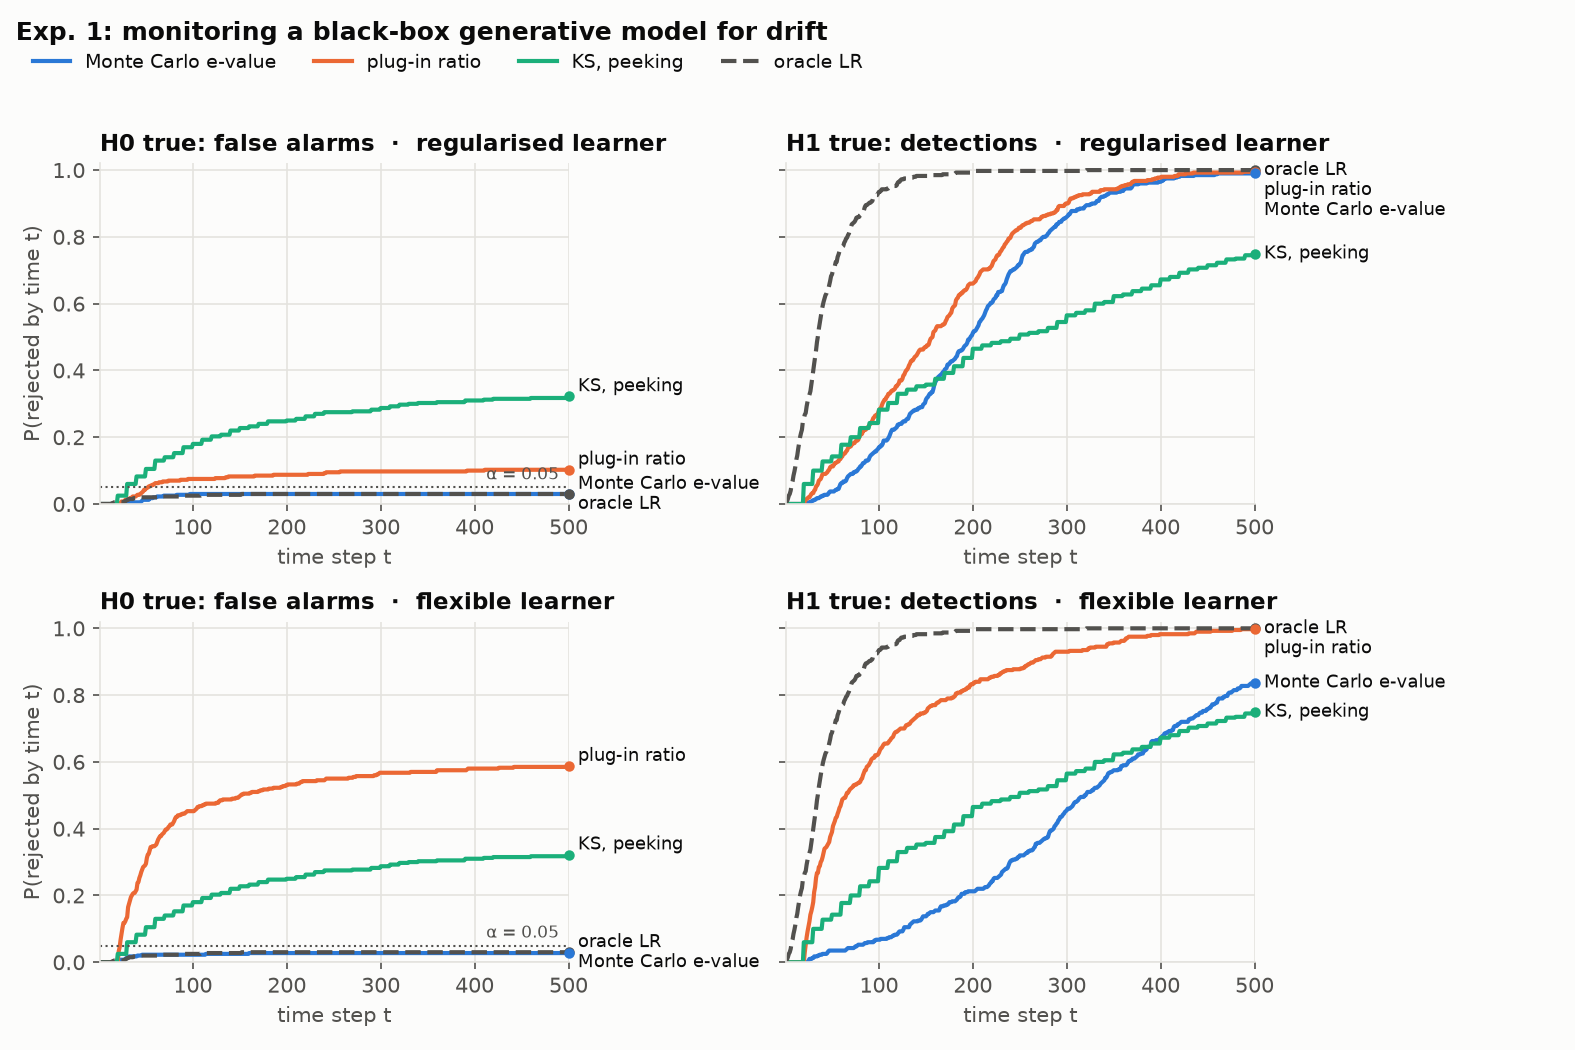
\includegraphics[width=\textwidth]{exp1_generative_drift.png}
\caption{Probability of having rejected by time $t$ in the generative-drift
experiment. Left: the null is true (false alarms). Right: the model has
drifted (detections). The dotted line is $\alpha = 0.05$.}
\label{fig:drift}
\end{figure}

Table~\ref{tab:drift} and Figure~\ref{fig:drift} show the central point of the
paper. With the same score, using the learned ratio directly as the bet gives
10\% false alarms with the regularised learner and 59\% with the overfitting
one. The Monte Carlo e-process gives 3\% with both. The worse learner costs
power, not validity. Recomputing a KS test every ten steps gives 32\% false
alarms. The oracle is far ahead (median 35 steps), which is the price of
learning the discrepancy online and the subject of
Sections~\ref{sec:exp-budget} and~\ref{sec:exp-blr}.

\subsection{An adaptive bandit checked against a digital twin}\label{sec:exp-bandit}

Three arms are allocated by Thompson sampling on the real outcomes. The twin
simulates any arm: $y = \mu_k + e^{\epsilon/2} - e^{1/8}$ with
$\epsilon \sim \mathcal N(0, 1)$ and $\mu = (0, 0.2, 0.4)$. Under the
alternative, arm 0 is better in reality than the twin predicts (mean shifted
by 0.5), so Thompson sampling moves towards it: it pulls arm 0 in 65\% of
steps, against 7\% under the null. Horizon 400. The score is a per-arm
quadratic logistic regression. We add the Monte Carlo e-process with the twin
run on \emph{uniformly random} arms instead of the chosen arm, which is the
setting of Proposition~\ref{prop:necessary}, and a per-arm Welch $t$-test
recomputed every ten steps.

\begin{table}[t]
\centering
\caption{Thompson-sampling bandit against a digital twin
(Section~\ref{sec:exp-bandit}).}
\label{tab:bandit}
\begin{tabular}{lrrr}
\toprule
method & false alarms & power & median stop \\
\midrule
MC e-process, twin run on the chosen arm & 0.028 & 1.000 & 49 \\
MC e-process, twin run on random arms & 1.000 & 1.000 & 40 \\
plug-in & 0.055 & 1.000 & 44 \\
per-arm $t$-test, recomputed & 0.388 & 1.000 & 30 \\
oracle LR & 0.043 & 1.000 & 15 \\
\bottomrule
\end{tabular}
\end{table}

\begin{figure}[t]
\centering
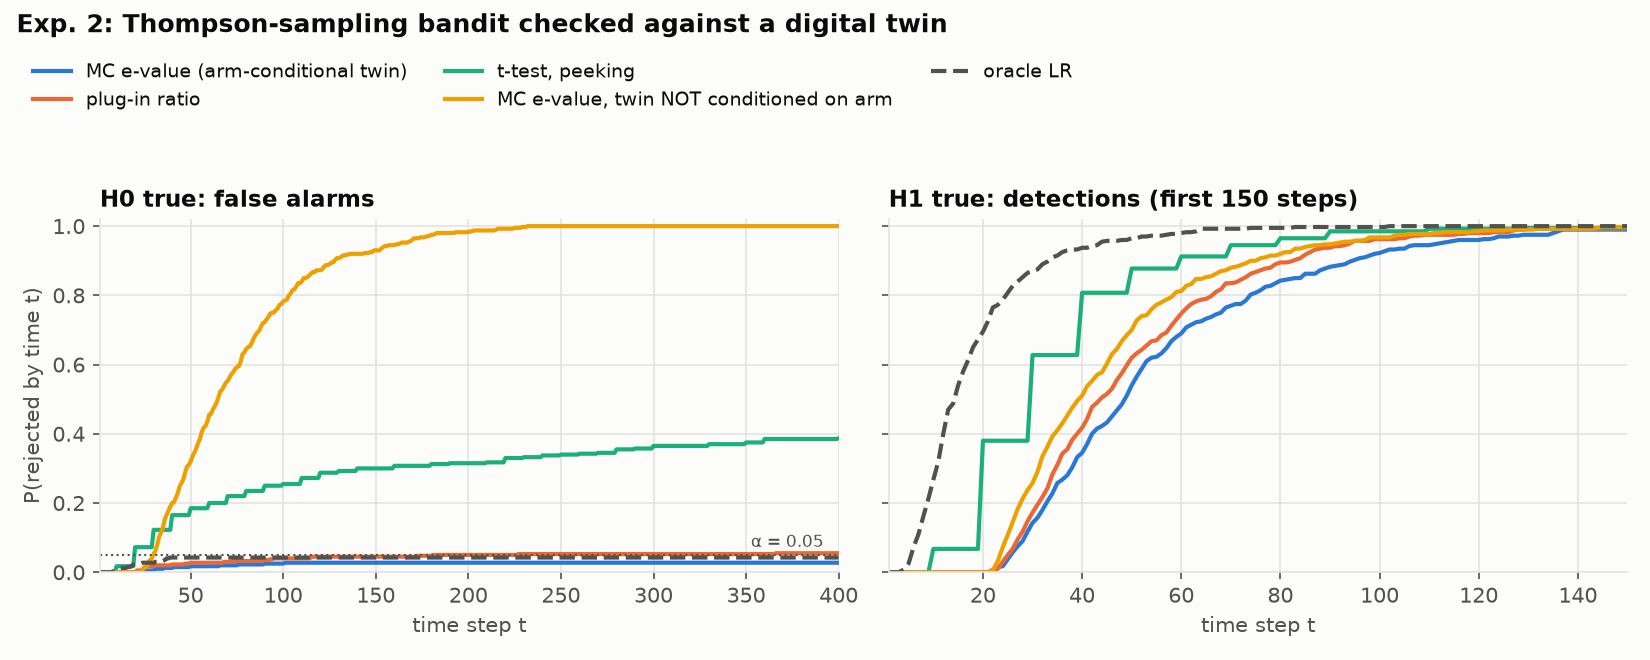
\includegraphics[width=\textwidth]{exp2_adaptive_bandit.png}
\caption{Bandit experiment. Simulating without conditioning on the chosen
arm rejects a true null in every run (Proposition~\ref{prop:necessary}).}
\label{fig:bandit}
\end{figure}

Adaptive allocation does not affect the conditioned e-process: its false-alarm
rate is 2.8\% (Table~\ref{tab:bandit}). The unconditioned version rejects the
true null in every run, in most runs within the first hundred steps
(Figure~\ref{fig:bandit}). Thompson sampling concentrates on the best arm, so
the real outcomes follow that arm's law while the simulated ones follow a
mixture over arms, exactly as in Proposition~\ref{prop:necessary}. The
recomputed $t$-test has 39\% false alarms. Here the plug-in happens to be
nearly calibrated (5.5\%), but nothing guarantees this.

\subsection{Simulation budget and the growth theory}\label{sec:exp-budget}

\begin{table}[t]
\centering
\caption{Simulation budget in the drift experiment (regularised learner, 200
replications).}
\label{tab:budget}
\begin{tabular}{lrrrrrr}
\toprule
$M$ & 1 & 2 & 4 & 8 & 16 & 64 \\
\midrule
false alarms & 0.030 & 0.030 & 0.035 & 0.030 & 0.020 & 0.015 \\
power & 0.780 & 0.960 & 0.990 & 0.990 & 0.995 & 1.000 \\
median stop & 371 & 282 & 227 & 212 & 202 & 207 \\
\bottomrule
\end{tabular}
\end{table}

Table~\ref{tab:budget} varies $M$. Validity holds at every budget, including
$M = 1$. The median stopping time at $M = 1$ is 1.8 times that at $M = 64$,
close to the factor 2 predicted by Theorem~\ref{thm:growth}(iv). For larger $M$
the observed ratios are smaller than predicted, as expected when part of the
stopping time is spent learning the score.

\begin{figure}[t]
\centering
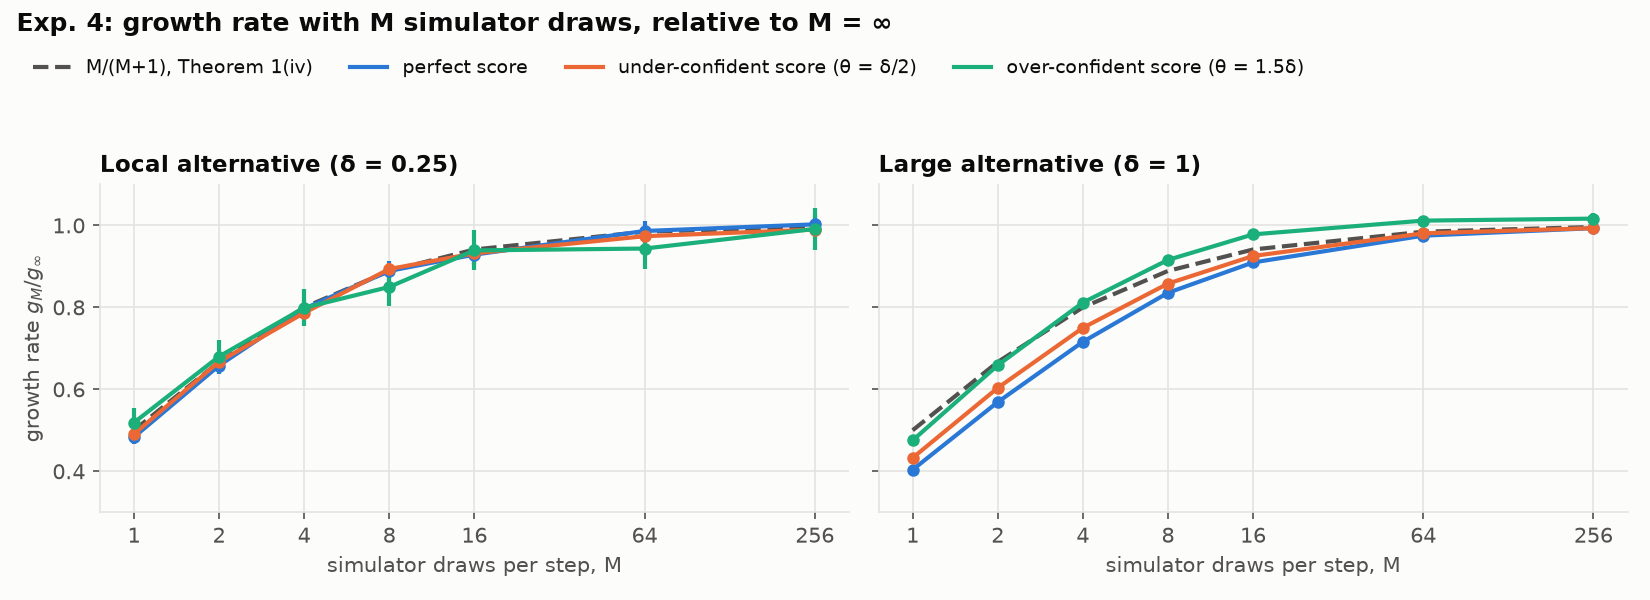
\includegraphics[width=\textwidth]{exp4_growth_rate.png}
\caption{Growth rate $g_M$ relative to $g_\infty$ for $P = \mathcal N(0,1)$,
$Q = \mathcal N(\delta, 1)$ and score $T(x) = e^{\theta x}$, estimated from
$4 \times 10^5$ draws (two standard errors shown). Dashed: $M/(M+1)$ from
Theorem~\ref{thm:growth}(iv).}
\label{fig:growth}
\end{figure}

To check Theorem~\ref{thm:growth} directly we take $P = \mathcal N(0, 1)$,
$Q = \mathcal N(\delta, 1)$ and $T(x) = e^{\theta x}$, for which
$\hat Q = \mathcal N(\theta, 1)$, $g_\infty = \theta\delta - \theta^2/2$ and
$\rho = e^{\theta\delta}$ are explicit. Figure~\ref{fig:growth} shows the
results:
\begin{itemize}
  \item The ceiling (i) and the lower bound (iii) hold in all 56
        configurations (within three Monte Carlo standard errors). The lower
        bound is conservative.
  \item For $\delta = 0.25$ the efficiency $g_M/g_\infty$ is 0.48, 0.66,
        0.80, 0.89 and 0.93 at $M = 1, 2, 4, 8, 16$, against
        $M/(M+1) = 0.50, 0.67, 0.80, 0.89, 0.94$, for perfect, under- and
        overconfident scores alike.
  \item For $\delta = 1$ a perfect score does worse than $M/(M+1)$ at small $M$.
  \item With $\theta = 2\delta$ and $\delta = 1$, where $g_\infty = 0$, the
        growth rate rises to 0.18 at $M = 4$ and then falls towards zero as $M$
        grows: a finite budget tempers an overconfident score.
\end{itemize}

\subsection{Updating the score at every step}\label{sec:exp-blr}

We replace the refitted point estimate by the online Bayesian learning rule
\eqref{eq:blr}, updated at every step with no burn-in, and bet either with the
posterior predictive log-odds $\kappa\mu$ or with the posterior mean $\mu$.
Features are standardised using simulator draws only. Seeds are as in
Sections~\ref{sec:exp-drift}--\ref{sec:exp-bandit}, so the real data are
identical.

\begin{table}[t]
\centering
\caption{Refitted point estimate versus the online Bayesian learning rule (BLR),
400 replications, MC e-process throughout.}
\label{tab:blr}
\begin{tabular}{llrrr}
\toprule
task & score & false alarms & power & median stop \\
\midrule
drift, degree 4 & refitted point estimate & 0.030 & 0.990 & 198 \\
 & BLR, posterior mean & 0.030 & 0.965 & 238 \\
 & BLR, predictive & 0.018 & 0.983 & 209 \\
drift, degree 6 & refitted point estimate & 0.028 & 0.838 & 320 \\
 & BLR, posterior mean & 0.033 & 0.940 & 242 \\
 & BLR, predictive & 0.015 & 0.965 & 214 \\
bandit & refitted point estimate & 0.028 & 1.000 & 49 \\
 & BLR, posterior mean & 0.025 & 1.000 & 51 \\
 & BLR, predictive & 0.030 & 1.000 & 38 \\
\bottomrule
\end{tabular}
\end{table}

\begin{figure}[t]
\centering
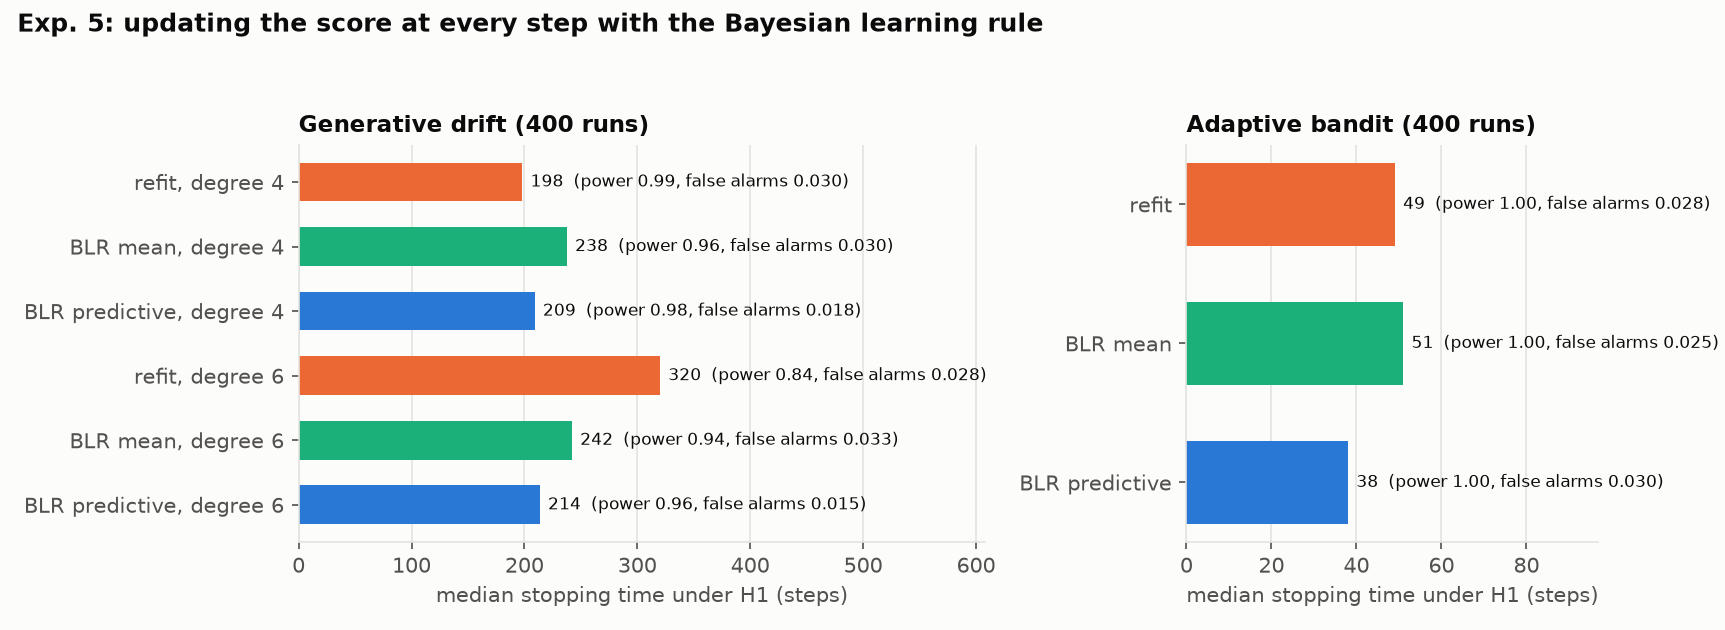
\includegraphics[width=\textwidth]{exp5_bayesian_learning_rule.png}
\caption{Median stopping time under the alternative, by score, with power
and false-alarm rates.}
\label{fig:blr}
\end{figure}

Table~\ref{tab:blr} and Figure~\ref{fig:blr} show three effects:
\begin{itemize}
  \item The posterior predictive beats the posterior mean in every setting,
        as the tempering result of Section~\ref{sec:power} suggests.
  \item It makes the method insensitive to the flexibility of the features:
        with degree 6, power rises from 0.84 to 0.97 and the median stopping
        time falls from 320 to 214, close to the degree-4 value.
  \item It is the fastest score in the bandit (38 against 49 steps) and on
        par with refitting for well-regularised features (209 against 198),
        without refitting.
\end{itemize}
False alarms stay between 1.5\% and 3.3\%. The posterior does not make the
plug-in valid: using the BLR odds directly as the bet gives between 14\% and
74\% false alarms.

%======================================================================
\section{Related work}\label{sec:related}
%======================================================================

\paragraph{Monte Carlo tests.} Classical Monte Carlo tests compare a fixed
dataset with simulations from the null \citep{besag1989generalized}.
\citet{fischer2024sequential} make them anytime-valid in the number of
simulations for a fixed dataset, in order to save computation, and
\citet{barber2026montecarlo} give guarantees without exact joint
exchangeability. In our setting the data themselves arrive over time, and
fresh simulations are drawn for each new observation.

\paragraph{Besag--Clifford e-values.} \citet{dombowsky2026besag} construct
e-values from samples that are exchangeable with the data under the null,
generated by parallel Markov chains, for models with intractable normalising
constants. They prove log-optimality as the number of samples grows, and they
list generative-model evaluation and sequential testing among the
applications. This is the closest work to Proposition~\ref{prop:exact} and to
parts of Theorem~\ref{thm:growth}. Our focus differs in three respects:
\begin{itemize}
  \item a data stream under adaptive control, with the necessity result of
        Proposition~\ref{prop:necessary};
  \item arbitrary learned scores, analysed through the tilted null;
  \item the explicit finite-budget constant $M/(M+1)$.
\end{itemize}
The precise overlap should be settled against their full text.

\paragraph{Sequential tests with a sampled null.} Model-X sequential testing
of conditional independence \citep{shaer2023modelx} draws, at each step, a
dummy covariate from its known conditional law and bets on a learned
predictor. The mechanism is the same as ours with $M = 1$, applied to a
different null. Sequential predictive two-sample tests bet with an online
classifier separating two streams
\citep{podkopaev2023sequential,shekhar2023nonparametric}. The sequential
kernelised Stein discrepancy tests goodness of fit for unnormalised densities
but needs the score function \citep{martinez2025sequential}. Conformal test
martingales \citep{vovk2003testing,vovk2021testing} and their weighted
versions for monitoring deployed AI systems \citep{prinster2025watch} test the
exchangeability of the stream, with no reference model.

\paragraph{Adaptively collected data.} Randomisation tests for adaptively
collected data \citep{nair2023randomization}, the randomisation e-process for
trial monitoring \citep{zampieri2025sequential}, anytime-valid off-policy
inference \citep{waudbysmith2024anytime} and adaptive auditing of AI systems
\citep{zhou2026adaptive} all handle adaptivity, but none of them uses a
simulator as the null. Digital-twin validation by re-initialising the twin
from observed states and simulating conditionally on part of the trace
\citep{ghasemloo2026subtrace} uses the same conditioning idea with
fixed-sample tests.

\paragraph{Bayesian updating.} The score update is an instance of the Bayesian
learning rule \citep{khan2023bayesian}, in the one-step online form of
\citet{jones2024bong}. The link between predictive scores and Bayes factors
is the prequential view of the marginal likelihood
\citep{clarke1990information}.

%======================================================================
\section{Discussion}\label{sec:discussion}
%======================================================================

The Monte Carlo e-process separates two concerns that are usually entangled.
Validity comes from exchangeability with fresh, correctly conditioned
simulations, and holds for any score and any policy. Power comes from the
score, and Theorem~\ref{thm:growth} measures it by the distance between the
tilted null and the truth, scaled by $M/(M+1)$. Approximations made when
computing the score, such as variational posteriors or single-step updates,
can therefore cost power but never validity.

Several limitations remain.
\begin{itemize}
  \item \textbf{Simple conditional nulls only.} Simulators with unknown
        calibration parameters need composite-null constructions, such as
        universal inference or reverse information projections
        \citep{grunwald2024safe}, adapted to samplers.
  \item \textbf{Approximate simulators.} MCMC-based samplers break exact
        exchangeability; the guarantees of \citet{barber2026montecarlo}
        suggest how to control the resulting error.
  \item \textbf{A cumulative bound for approximate posteriors is missing.}
        Proposition~\ref{prop:bayes} treats exact posteriors with an unlimited
        budget; a bound for the online Bayesian learning rule with finite $M$
        is open.
  \item \textbf{Low-dimensional experiments.} High-dimensional generative
        models call for learned feature maps and structured posterior
        approximations.
\end{itemize}

\paragraph{Reproducibility.} Code, results and figures are in the repository
\texttt{evalues4generative}. All runs are seeded.

\bibliographystyle{plainnat}
\bibliography{references}

\appendix

%======================================================================
\section{Proofs}\label{app:proofs}
%======================================================================

\paragraph{Proof of Theorem~\ref{thm:growth}.}
(i) Under $H_0$ the pair $(X, Y_{1:M})$ has law $P \otimes P^M$, under which
$E^{(M)}$ has expectation one. The likelihood ratio of $Q \otimes P^M$ to
$P \otimes P^M$ is $(dQ/dP)(X)$. By Jensen's inequality,
$\E_{Q \otimes P^M}[\log E^{(M)} - \log(dQ/dP)(X)] \le
\log \E_{P \otimes P^M}[E^{(M)}] = 0$.

(ii) By the strong law of large numbers, $M^{-1}\sum_j T(Y_j) \to Z$ almost
surely, so $E^{(M)} \to T(X)/Z = (d\hat Q/dP)(X)$. Moreover
$\log(d\hat Q/dP) = \log(dQ/dP) - \log(dQ/d\hat Q)$; take expectations under $Q$.

(iii) Let $S = \sum_j T(Y_j)$. Then
$\log E^\infty - \log E^{(M)} = \log\{(T(X) + S)/((M+1)Z)\}$. Conditioning on $X$
and applying Jensen's inequality over $Y_{1:M}$,
\[
\E\big[\log E^\infty - \log E^{(M)} \mid X\big]
\le \log\frac{T(X) + MZ}{(M+1)Z}
= \log\Big(1 + \frac{T(X)/Z - 1}{M+1}\Big)
\le \frac{T(X)/Z - 1}{M+1}.
\]
Taking the expectation under $Q$ gives $g_\infty - g_M \le (\rho - 1)/(M+1)$.

(iv) Let $Z_0 = X$ and $Z_k = Y_k$, and let $\bar h$ and $\overline{h^2}$ be
the averages of $h(Z_k)$ and $h(Z_k)^2$ over $k = 0, \ldots, M$. The cumulant
expansion of $\log$ of the average of $e^{\varepsilon h(Z_k)}$ gives
\[
\log E^{(M)} = \varepsilon\big(h(X) - \bar h\big)
- \frac{\varepsilon^2}{2}\big(\overline{h^2} - \bar h^2\big) + O(\varepsilon^3).
\]
Under $Q \otimes P^M$,
$\E[h(X) - \bar h] = \frac{M}{M+1}(\E_Q h - \E_P h)
= \frac{M}{M+1}\,\varepsilon\, \E_P[\tilde h g]$. The second bracket is the
empirical variance of $M+1$ draws that are i.i.d.\ $P$ up to $O(\varepsilon)$,
with expectation $\frac{M}{M+1}\mathrm{Var}_P(h) + O(\varepsilon)$. Hence
$g_M = \frac{M}{M+1}\varepsilon^2\big(\E_P[\tilde h g] - \frac12 \E_P[\tilde h^2]\big)
+ O(\varepsilon^3)$, which equals the stated form since $\E_P[g] = 0$. The
expansion of $\KL(Q\|P)$ is standard.

\paragraph{Proof of Proposition~\ref{prop:bayes}.} By Fubini,
$\E_P[T_t] = \int \E_P[dQ_\theta/dP]\,\pi_{t-1}(d\theta) = 1$, so by
Theorem~\ref{thm:growth}(ii) $E_t^\infty = T_t(X_t)$. Writing
$q_\theta = dQ_\theta/dP$, the posterior predictive ratio is
$T_t(x) = \int q_\theta(x) \prod_{i<t} q_\theta(X_i)\,\pi_0(d\theta) \big/
\int \prod_{i<t} q_\theta(X_i)\,\pi_0(d\theta)$, and the product over $t$
telescopes to the marginal likelihood ratio. The Laplace expansion under
regularity conditions is \citet{clarke1990information}. Finally
$\E_Q[\log q_\theta] = \KL(Q\|P) - \KL(Q\|Q_\theta)$.

%======================================================================
\section{Experimental details}\label{app:details}
%======================================================================

\paragraph{Refitted learner.} Balanced logistic regression on standardised
monomials of the observation (degree 4 or 6; for the bandit, per-arm terms
$1, y, y^2$), with a ridge penalty on all coefficients except the intercept.
It is refitted by eight Newton steps on all real observations and up to the
last 4000 simulator draws, every ten steps from step 20; until the first fit
the score is zero and $E_t = 1$.

\paragraph{BLR learner.} The same model, with prior $\mathcal N(0, I)$ on the
standardised coefficients and variance 10 on the intercept. Features are
standardised with 2000 (bandit: 3000) simulator draws from a stream
independent of the data. At each step, the real observation has weight one
and each of the $M$ simulator draws weight $1/M$, and expectations under the
current posterior use the probit approximation. Scores are clipped to
$[-30, 30]$ for both learners.

\paragraph{Seeds and cost.} Replication $i$ uses seed $i$ under the null and
$10^6 + i$ under the alternative, for every method, so methods are compared
on identical real data. On four cores, the drift experiment takes about one
minute per 400 replications with the regularised learner and four minutes
with the flexible one; the full set of experiments takes under an hour.

\end{document}
